\section {Signal Characterization and Test Procedures}

In domestic ISDB-T receivers It is not commonly possible to perform bit error rate measures. Thus, new methods were proposed by ITU (Texti{international Telecommunications Union}) to establish the protection relationship, and to ensure the quality of service. The criterion chosen in this study to determine the point of failure was based on the recommendation ITU-R BT. 1368-12 cite{ITU_BT_1368}, where the protection relationship is determined subjectively through the evaluation of image quality. par
%=========================================================

The application of the method was performed by varying the level of the interfering signal, while the image received was observed. The level of the primary service was kept constant, at a pre-established value, while the level of the interfering signal was increased to the point where it became noticeably noticeable constant errors or image freezing, regardless of the visual acuity of the Observer. It was used, as recommended, that the limit condition occurs when there are no errors in the image in the first 20 seconds of observation. par
%=========================================================

The tests performed consider that the channels are spaced at 428.571 KHz, as illustrated in Figure ref{fig: ISDB_channel_Spacing} cite{ARIB_STD_B31} and cite{NBR_15601}. To measure the channel power was adopted 6MHz and 18MHz of integration bandwidth, with resolution of 100KHz. \par

\begin{figure}[h!]
    \centering
    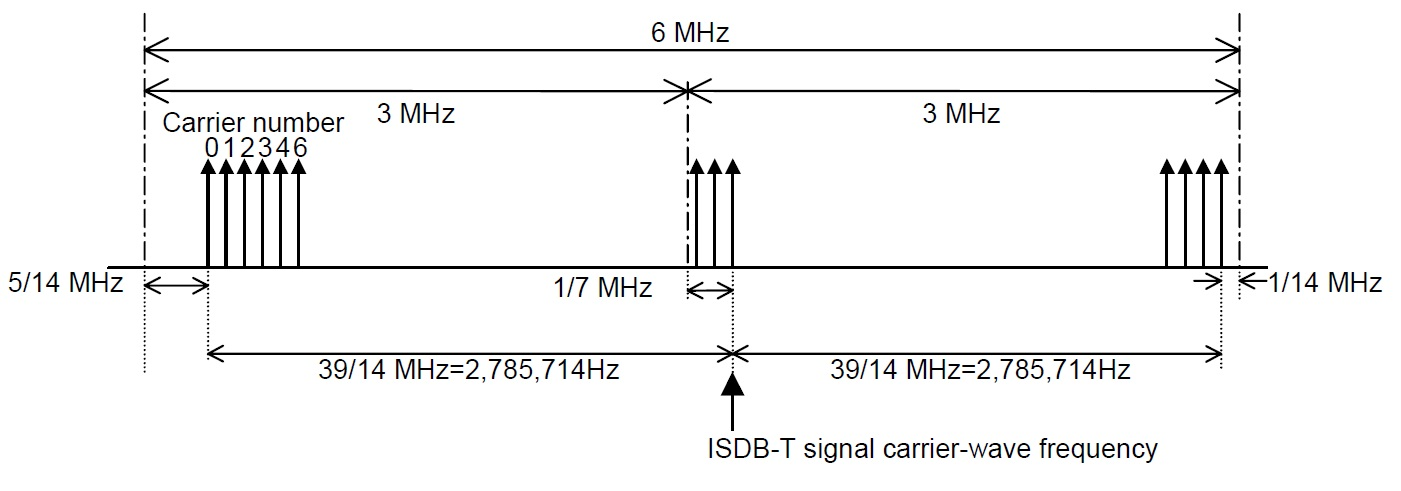
\includegraphics[width=0.45\textwidth]{Figures/Arib_ISDB_T_channel_Spacing}
    \caption{ISDB-T channel spacing}
    \label{fig:ISDB_channel_Spacing}
\end{figure}

%=========================================================
\subsection{ISDB-T Signal characterization}
%=========================================================

The characterization of the digital TV signal used in the tests was performed according to the parameters presented in table ~ ref{tab: table_ISDBT}. par
%=========================================================

\begin{table}[h!]
	\begin{center}
		\centering
		\caption{Caracterização do sinal de ISDB-T usado nos testes laboratoriais.}
		\label{tab:table_ISDBT}
		\begin{tabular}{|l|c|c|c|}
			\hline
			\textbf{Camada} & \textbf{A} & \textbf{B} & \textbf{C}\\
			\hline
			Número de segmentos & 13 & - & -\\
			\hline
			Modulação & 64QAM & - & -\\
			\hline
			FEC & 3/4 & - & -\\
			\hline
			Entrelaçamento no Tempo & 2 & - & -\\
			\hline
			Largura de banda &\multicolumn{3}{c|}{5,572421MHz}\\
			\hline
			Recepção Parcial &\multicolumn{3}{c|}{Não}\\
			\hline
			Modo &\multicolumn{3}{c|}{\textit{Mode} 3}\\
			\hline
		    Intervalo de Guarda &\multicolumn{3}{c|}{1/8}\\
			\hline
		\end{tabular}
	\end{center}
\end{table}
%=========================================================

\subsection {Ajuste do limiar de recepção dos receptores ISDB-T}
%=========================================================

The receiving threshold expresses the level in dBm under which the receiving test must operate throughout the tests. The following procedures were adopted to determine the receiving threshold cite{LTE_ISDBT}. par


\begin{enumerate}[label=(\alph*)]
    %a
    \item Aplicou-se um vídeo TS de referencia, na respectiva entrada do modulador.
    %b
    \item Ajustou-se o sinal de TVD para o canal 32 UHF, inicialmente com o nível de -70 dBm e modulação 64QAM, caracterizado conforme descrito na tabela \ref{tab:table_ISDBT}. Conferiu-se se o video estava sendo exibido sem falhas pelo receptor em teste.
    %c
	\item O nível do sinal de TVD foi reduzido até que houvesse falha visível e constante na imagem, independente da acuidade visual do observador. Observou-se a estabilização da qualidade da imagem por pelo menos 20s, conforme determina \cite{ITU_BT_1368}.
    %d
    \item O nível foi conferido utilizando analisador digital se sinais, no modo de medição de potência de canal.Partindo do limiar de visibilidade, o nível  do sinal foi aumentado em 3 dB.
    %e
    \item Os itens de (a) a (e) foram então repetidos para todos os receptores.
\end{enumerate}

%=========================================================
%\begin{table}[h!]
%	\begin{center}
%		\centering
%		\caption{Nível de operação dos receptores ISDB-T.}
%		\label{tab:Receptores}
%		\begin{tabular}{|l|c|c|c|c|}
%			\hline
%			\textbf{Receptor} & \textbf{RX1} & \textbf{RX2} & \textbf{RX3} & \textbf{RX4}\\
%			\hline
%			Nível (dBm/6MHz)&-75,7 & -75,2 & -79,7 & -75,1\\
%			\hline
%			Nível (dBm/18MHz)&-75,2 & -73,7 & -77,9 & -73,8\\
%			\hline
%		\end{tabular}
%	\end{center}
%\end{table}
%=========================================================

\subsection{Interferência em canal adjacente}

The objective of this experiment is to establish the harmful interference point for operation in adjacent channels, by determining the saturation threshold (the $ _{th} $) that expresses the power in dBm from the TVD receiver loses the ability to discriminate The interferent signal of the desired. The following steps were performed to perform this assay, par  
%=========================================================

\begin{enumerate}[label=(\alph*)]
    \item   O sinal ISDB-T caracterizado anteriormente foi ligado ao arranjo de medidas.
    \item 	Aplicou-se inicialmente um sinal interferente modulado com a tecnologia OFDM operando no canal adjacente inferior ($N$-1).  
    \item 	A potência do sinal interferente foi aumentada em passos de 0,5dB até que a imagem analisada apresentasse erros constantes.
    \item 	Ao atingir a condição limite, a potência do canal adjacente foi medida.
    \item 	Repetiu-se os procedimentos (a) até (d) variando entre as tecnologias GFDM, W-GFDM e F-OFDM.
    \item 	Por fim, repetiu-se os itens (a) até (e) operando agora no canal adjacente superior ($N$+1).
\end{enumerate}
%=========================================================

The characterization used is shown in the table ref{tab: table_ADJ_01}.
%=========================================================

\begin{table}[h!]
	\begin{center}
		\centering
		\caption{Configuração dos sinais interferente para teste de interferência  em canais adjacentes.}
		\label{tab:table_ADJ_01}
		\begin{tabular}{|l|c|c|c|c|}
			\hline
			\textbf{} & \textbf{OFDM} & \textbf{GFDM} & \textbf{W-GFDM} & \textbf{F-OFDM}\\
			\hline
			$M$ & 1 & 3 & 3 & 1\\
			\hline
			$K$ &\multicolumn{4}{c|}{512}\\
			\hline
			$KoffS$ &\multicolumn{4}{c|}{128}\\
			\hline
			$KoffC$ &\multicolumn{4}{c|}{0}\\
			\hline
			$nCP$ &\multicolumn{4}{c|}{64}\\
			\hline
			$nCS$ & 0 & 0 & 50 & 0\\
			\hline
			$nW$ & 0 & 0 & 50 & 0\\
			\hline
		\end{tabular}
	\end{center}
\end{table}
%=========================================================

\newenvironment{conditions*}
  {\par\vspace{\abovedisplayskip}\noindent
   \tabularx{\columnwidth}{>{$}l<{$} @{${}={}$} >{\raggedright\arraybackslash}X}}
  {\endtabularx\par\vspace{\belowdisplayskip}}

Onde:

\begin{conditions*}

M & Sub símbolos \\
K & Total de portadoras\\   
KoffS & Portadoras desligadas lateralmente\\
KoffC & Portadoras desligadas ao centro\\
nCp & Amostras de prefixo cíclico\\
nCp & Amostras de sufixo cíclico\\
nW  & Amostras de janela\\
\end{conditions*}

%\begin{conditions*}
%M & N\textsuperscript{\underline{o}} de sub símbolos \\
%K & N\textsuperscript{\underline{o}} total de portadoras\\   
%KoffS & N\textsuperscript{\underline{o}} de portadoras desligadas lateralmente\\
%KoffC & N\textsuperscript{\underline{o}} de portadoras desligadas no centro do sinal\\
%nCp & N\textsuperscript{\underline{o}} de amostras de prefixo-cíclico\\
%nW  & N\textsuperscript{\underline{o}} de amostras da janela\\
%\end{conditions*}

\subsection{Interferência com sinal operando canais associados e portadoras desligadas}
%=========================================================

One of the features of 5G waveforms designed for this assay is the ability to disconnect the central carriers, thus allowing the association of multiple idle channels. The proposed experiment intends to evaluate the ability of 5G waveforms to occupy multiple channels, without generating interferences in the existing primary services. par% An example of this scenario is illustrated in Figure ref{fig: setupLabview2}. 
The same procedures of the previous experiment were adopted, with the difference that to perform the power measurements, the ISDB-T signal was first disconnected. The characterization of this procedure is described in the table ref{tab: table_ADJ_02}. par
%=========================================================

\begin{table}[h!]
	\begin{center}
		\centering
		\caption{Caracterização para ensaio em múltiplos canais adjacentes.}
		\label{tab:table_ADJ_02}
		\begin{tabular}{|l|c|c|c|c|}
			\hline
			\textbf{} & \textbf{OFDM} & \textbf{GFDM} & \textbf{W-GFDM} & \textbf{F-OFDM}\\
			\hline
			$M$ & 1 & 3 & 3 & 1\\
			\hline
			$K$ &\multicolumn{4}{c|}{512}\\
			\hline
			$KoffS$ &\multicolumn{4}{c|}{104}\\ 
			\hline
			$KoffC$ &\multicolumn{4}{c|}{152}\\ 
			\hline
			$nCP$ & 64 & 50 & 50 & 64\\
			\hline
			$nCS$ & 0 & 0 & 50 & 0\\
			\hline
			$nW$ & 0 & 0 & 50 & 0\\
			\hline
		\end{tabular}
	\end{center}
\end{table}

%\begin{figure}[h!]
%    \centering
%    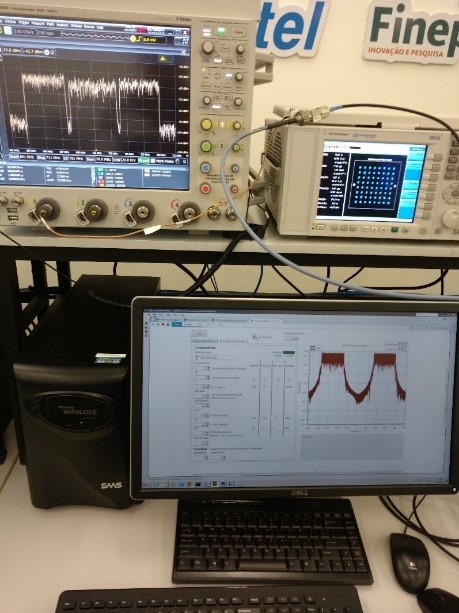
\includegraphics[width=0.25\textwidth]{Figures/setup_CRR.jpg}
%    \caption{Sinal 5G com canais associados e portadoras desligadas.}
%    \label{fig:setupLabview2}
%\end{figure}
